%\documentclass[11pt]{article}
%\usepackage{fullpage}

%\begin{document}

\subsection{Overview}
This section provides a detailed view over the system architecture and its components, describing them at both logical and physical level. \newline

\textbf{Section 2.2 - High-level components}: This subsection provides a description of high-level components and their interactions. \newline

\textbf{Section 2.3 - Component view}: This subsection provides a detailed insight of the components described in the previous section. \newline

\textbf{Section 2.4 - Deployment view}: This subsection provides a set of indications on how to deploy the illustrated components on physical tiers. \newline

\textbf{Section 2.5 - Runtime view}: In this subsection sequence diagrams are used to describe the way components interact to accomplish specific tasks typically related to your use cases. \newline

\textbf{Section 2.6 - Component interfaces}: This subsection provides a description of the different type of interfaces among the various described components. \newline

\textbf{Section 2.7 - Selected architectural styles and patterns}: This subsection provides a list of the architectural styles, design patterns and paradigms adopted in the design phase. \newline

\textbf{Section 2.8 - Other design decisions}: This subsection lists of all other relevant design decisions that were not mentioned before.

\clearpage

\subsection{High-level components}
The main high-level components of the system are:

\begin{itemize}
\item \textbf{Database}: The system data layer; it includes all structures and entities responsible for data storage and management. No application logic is found at this level, apart from the DBMS one that must guarantee the correct functioning of the data structures while assuring the ACID properties of transactional databases.

\item \textbf{Application Server}: This layer encloses all the logic for the system applications, including the logic needed to interface with external systems and the key algorithms.

\item \textbf{Mobile App Interface}: The client layer dedicated to mobile devices; it communicates directly with the Application Server and only includes presentation logic.

\item \textbf{Wearable App Interface}: The client layer dedicated to wearable devices equipped with WearOS (Android) and watchOS (Apple). The app requires to be installed also on a smartphone and to be paired via bluetooth. It just shows dinamically user's data.

\item \textbf{Script Interface}:  The client layer dedicated to third parties who need to get huge quantities of data: our application doesn't provide other visual interfaces besides the mobile one, but we allow companies to get data through scripts and HTTPS requests providing them libraries to include in order to allow the communication (authentication always required). The layer communicates directly with the Application Server.
\end{itemize}

The described components are structured in three layers, as shown in the following figure. It also includes the interaction with external systems, that is intended to happen at the level of the Application Server.

\begin{center}
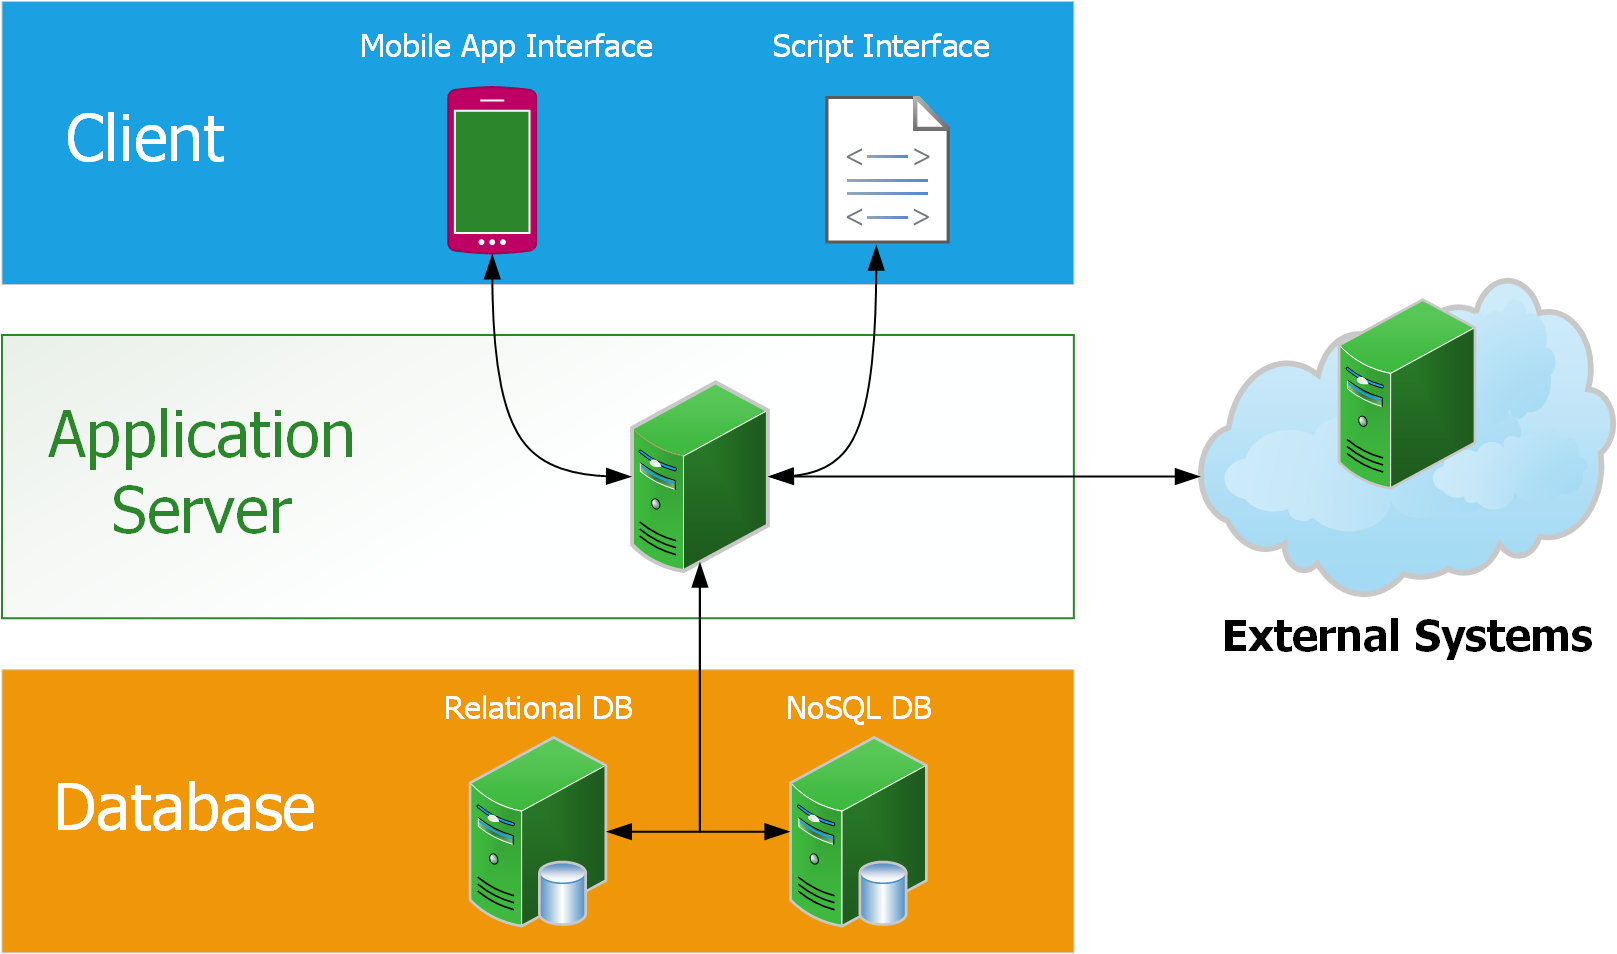
\includegraphics[scale=0.69]{sections/diagrams/layers.png}
\newline
\captionof{figure}{Logical layers of the system}
\end{center}

External systems are shown more in detail in the following figure: an high-level overview of the system components.

\begin{center}
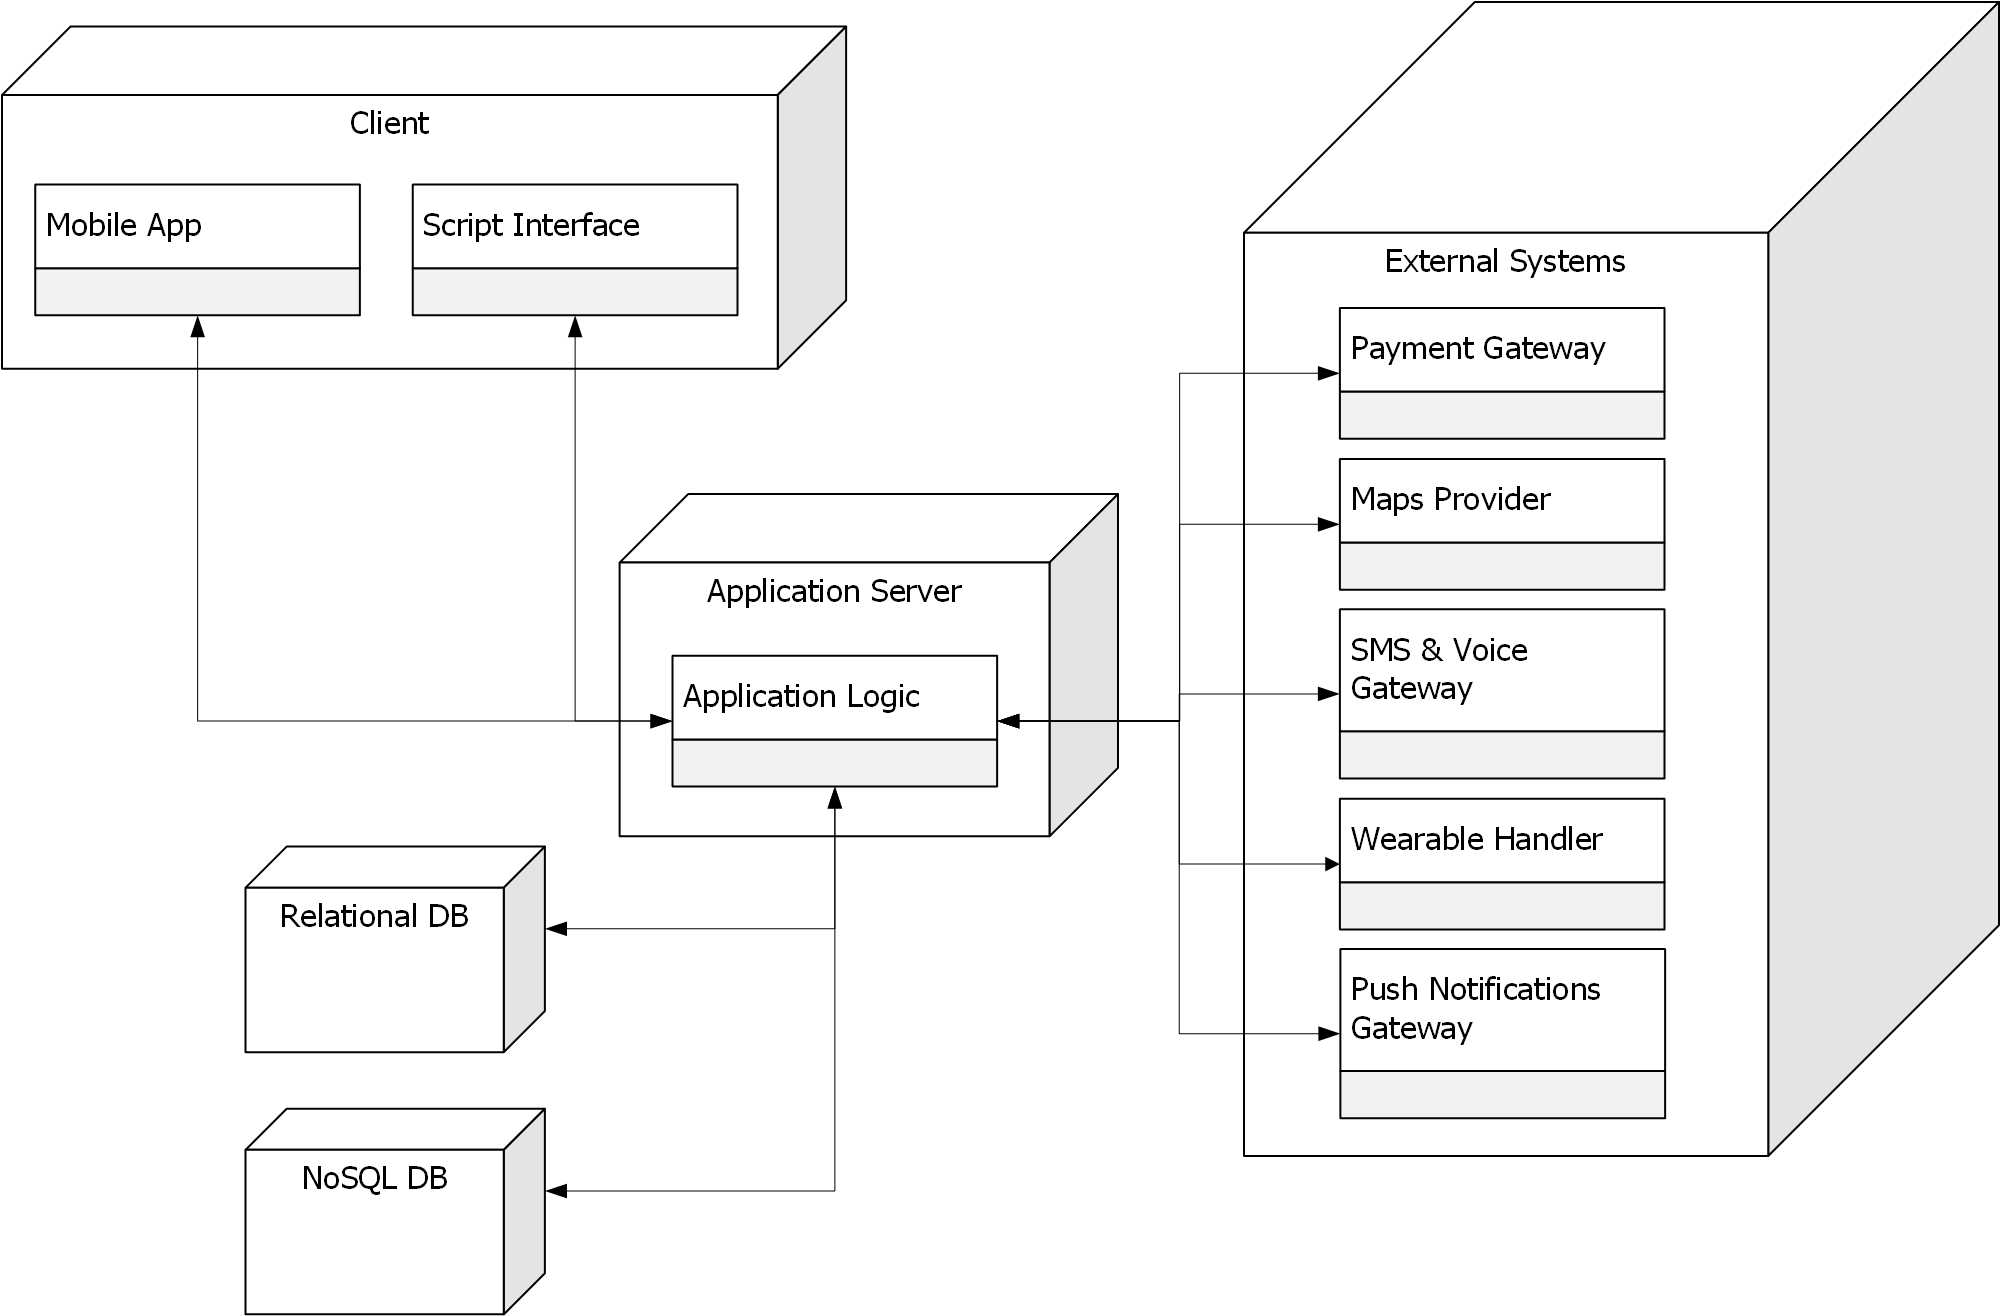
\includegraphics[scale=0.6]{sections/diagrams/highlevel.png}
\newline
\captionof{figure}{High-level components of the system}
\end{center}

\subsection{Component view}
\subsubsection{Database}
The Database layer must only be accessible through the Application Server via a dedicated interface. With respect to this, the Application Server must provide a persistence unit to handle the dynamic behaviour of all of the persistent application data. \newline

Besides the Database Engines, this layer is composed by a DBMS, which is in main part relational. The relational approach offers advantages ranging from the easy extensibility to independency from the physical organization, and in general the ACID properties of its transactions. For all these reasons fixed in front data and those that change less frequently are committed to the RDBMS, while for the others a NoSQL is provided. In fact thanks to its well-known scalability it fits better for data accumulated in large numbers every second, which is the case of all the data collected by the application through the wearable device. \newline

The Database layer has to store all the data shown in the following E-R diagram, the sensible of which must be encrypted before being stored.

\begin{center}
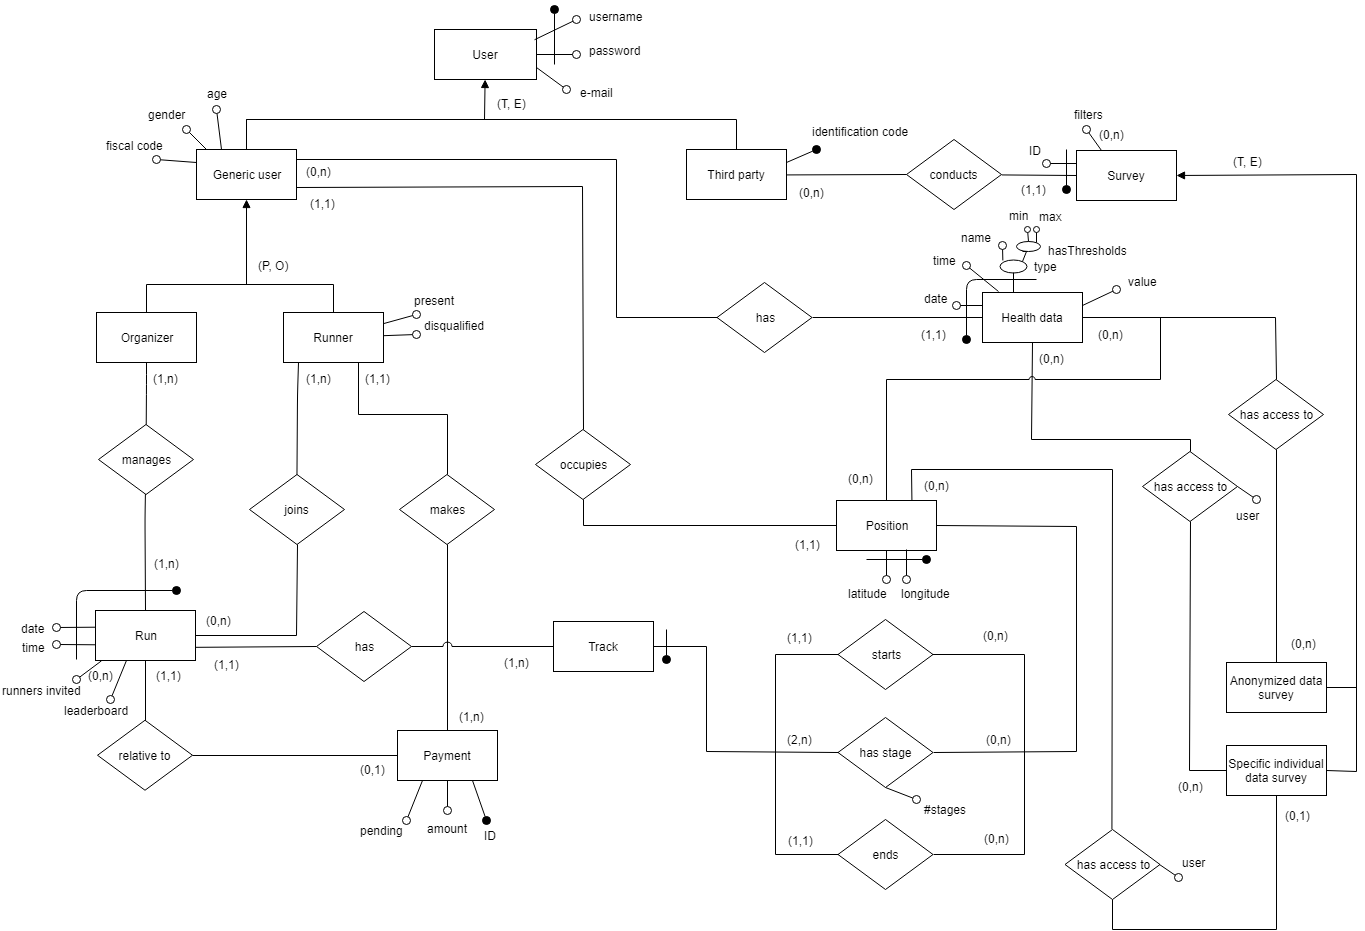
\includegraphics[scale=0.33]{sections/diagrams/ER.png}
\newline
\captionof{figure}{E-R model of the system}
\end{center}

\subsubsection{Application Server}
This layer must handle the business logic as a whole, the connections with the Database Layer and the multiple ways of accessing the application from different clients and external systems. The main feature of the Application Server are the specific modules of business logic, which describe business rules and work-flows for each of the functionalities provided by the application itself. \newline

The interface with the data layer must be handled, as stated before, by a dedicated persistence unit, that will be in charge of the object-relation mapping and dynamic data access and management; this ensures the fact that only the Application Server can access the Database. \newline

The Application Server must provide a means to interface with the mobile clients via specific APIs in order to decouple the different layers with respect to their individual implementation. Moreover, it must provide a way to communicate with external systems by adapting the application to the existing external infrastructures. \newline

The main business logic modules must include:
\begin{itemize}
\item \textbf{UserManager}: This module manages all the logic involved with user account management, login, registration and profile customization, as well as the generation and provision of user credentials. It also allows to visualize correctly the YOUR RACES screen.

\item \textbf{DataHandler}: This module manages the logic needed to manage data requests from third parties. It also includes the logic needed to communicate with external wearable devices and get data from them. It must also serve as an interface with the external Wearable Handler (e.g. Health app for iOS, Google Fit for Android, other available apps from various manufacturers).

\item \textbf{MapManager}: This module includes the logic needed to correctly visualize maps and markers moving on them, and also allows to choose and visualize stages. It must also serve as an interface with the external Maps Provider.

\item \textbf{PaymentGateway}: The logic involved in the computation of final charges is included in this module; moreover, this unit must stand as an interface with the external Payment Gateway upon the act of the automatic payments.

\item \textbf{EmergencyManager}: This module includes the logic needed to manage emergency calls and the sending of SMS. It must also serve as an interface with the external SMS \& Voice Gateway.

\item \textbf{NotificationManager}: This module serves as a gateway from the UserManager module, which needs to send an email to the clients, by managing the logic behind the email notification services. It also manages the logic needed to send and receive push notifications serving as an interface with the external Push Notifications Gateway.

\item \textbf{RunManager}: This module allows users to observe, participate, create and manage running races. It also has to provide and show info about races and it gets data from the MapManager, used to update leaderboards.
\end{itemize}

\subsubsection{Mobile Application Client}
As stated in the RASD document, the Mobile Application Client represents the main interface for customers and it should be implemented for both Android and iOS.

The mobile application must be designed in a way that makes communications with the Application Server easy and independent from the implementation of both sides. In order to do so, adequate APIs must be defined and used similarly to what has been described for the interactions between the two server layers.

The mobile application UI must be designed following the guidelines provided by the Android and iOS producers.

The mobile application directly communicates with the business logic using its RESTful API interfaces.

\subsubsection{Wearable Application Client}
As stated in the RASD document, the Wearable Application Client should be implemented for both WearOS and watchOS.

The software module to be included in the application must manage the GPS locations of the device and the connection with the device sensors, as well as the transmission of all health data to the mobile application via bluetooth.

\subsubsection{Desktop Client}
As mentioned before, currently TrackMe doesn't offer a desktop or web version of its application. However, companies can get data through scripts and HTTPS requests using provided libraries to include in order to allow the communication (authentication always required).

The Desktop Client directly communicates with the business logic of the Application Server.

\begin{center}
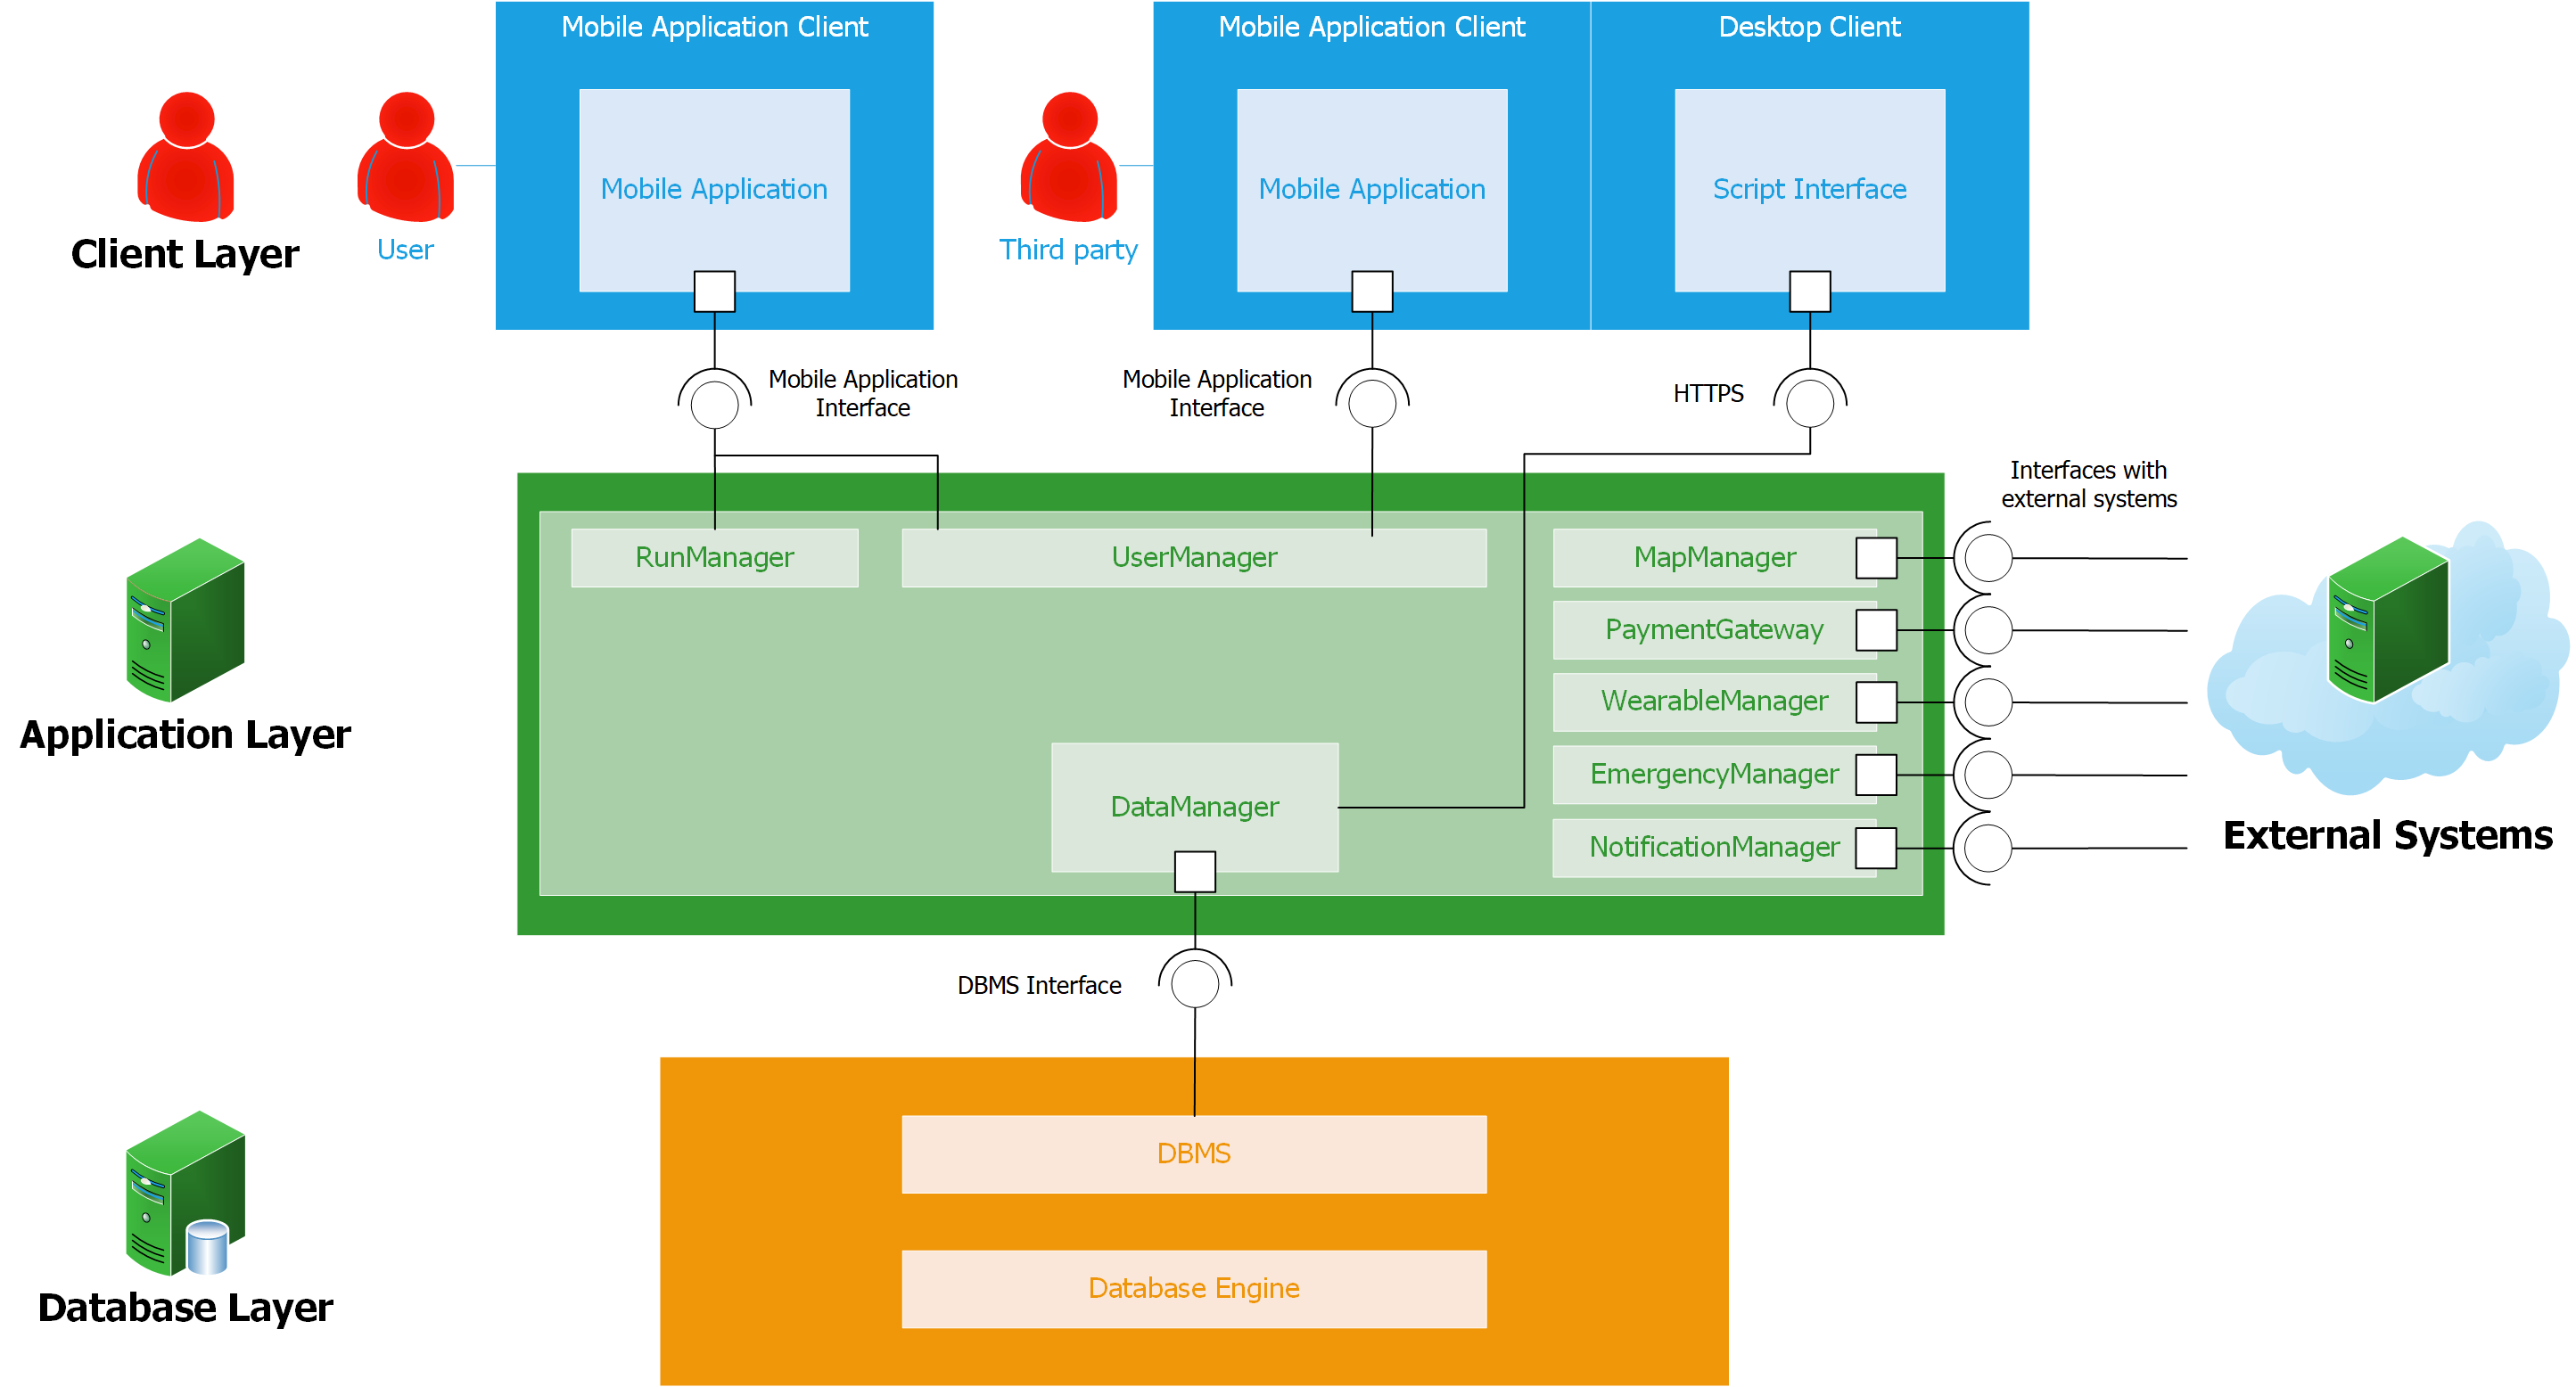
\includegraphics[scale=0.43]{sections/diagrams/globalCV.png}
\newline
\captionof{figure}{Global component view of the system}
\end{center}

\subsubsection{Implementation choices}
\paragraph{Database implementation}
The Database layer will be composed by two different databases: a relational database and a NoSQL database. The implementation choices for the relational one are the following:

\begin{itemize}
\item MySQL 5.7 as the relational DBMS.
\item InnoDB as the subsiding database engine; InnoDB is a good choice for this application, because it manages concurrent access to the same tables in a very clean and quick way.
\item The Java Persistence API (JPA) within the Application Server will serve as an interface with the Database.
\end{itemize}

The NoSQL Database is in charge of storing all the data generated by the system such as logs and all the kinds of data that  will not require any update or delete during the time and that will be accessed to consulted only. The decision of using a NoSQL database instead of a traditional relational database is driven by the need of speed in inserting and accessing a big amount of data. For this reason, it's not required to ensure all the ACID properties over transaction. The NoSQL Database runs on MongoDB as DBMS and communicates logic tier using TCP/IPO protocol on an arbitrary port. Also, the Eclipse JNoSQL interface is used for communications between the Application Server and the NoSQL Database.

Both databases must be physically protected and duplicated in order to avoid loss. Communication must be encrypted and different users should be created and assigned to the different softwares that access the database in order to always guarantee the minimum required level of privileges per software.

\paragraph{Application Server implementation}
The main choice for this layer is the use of Java Enterprise Edition 7 (JEE). This was the most reasonable option for several reasons. First of all, the final product is a large-scope application, and thus needs distribution to great numbers of clients simultaneously. For the same reason, it needs to satisfy continuously evolving functional requirements and customer demands. JEE also allows the developers to focus on the logic behind the main functionalities while being supported by a series of reliable APIs and tools that, among other features, can guarantee the main non-functional requirements of the case (e.g. security, reliability, availability...). Lastly, it can reduce the complexity of the application by using mechanisms and models that easily adapt to a large-scale project. 

The specific implementation choices are:

\begin{itemize}
\item GlassFish Server as the Application Server implementation.
\item Enterprise JavaBeans (EJB) to implement the single business logic modules described in the sections above using Stateless Beans. These will be appropriately subdivided into EJB containers as specified by the JEE documentation.
\item Java Persistence API (JPA) as persistence unit to perform the Database access, that is not implemented with direct SQL queries. Entity beans will be used to implement the object representation of the database entities and they are strictly related to the entities of the E-R diagram.
\item JAX-RS to implement proper RESTful APIs to interface with clients.
\item To interface with external systems, existing RESTful APIs defined by the partners will be used in the communication with the payment handlers, whereas a dedicated one will be provided to the maintenance system to interact properly with the application services.
\end{itemize}

\begin{center}
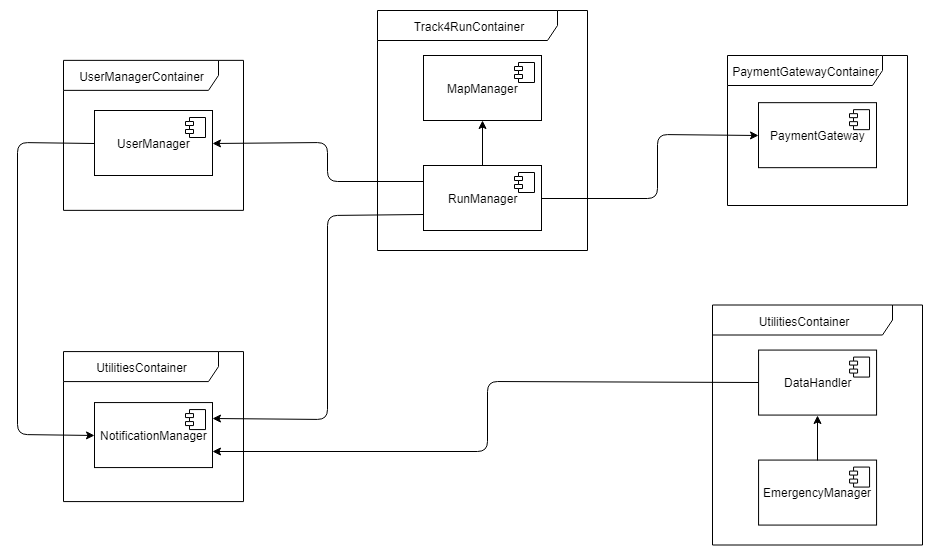
\includegraphics[scale=0.5]{sections/diagrams/component_view.png}
\newline
\captionof{figure}{The components of the Application Server	implemented as session beans to develop the business logic. An arrow going from component C1 to component C2 means that C1 uses interfacing methods provided	by C2}
\end{center}

\paragraph{Mobile Application Client implementation}
The mobile application UI must be designed following the design guidelines provided by the devices’ manufacturers. Two architectures must be supported: iOS and Android. The iOS application must be written in Swift, while the Android one must be implemented in Java.

The core of both application must be a Controller that communicates user inputs (after translating them from the UI input) to the Application Server via RESTful APIs. The access to the GPS of the devices and HealthData of users (only for devices that can collect these kind of data) must be performed through the default frameworks of the respective systems.

If the smartphone is paired with a device equipped with WearOS or watchOS with the TrackMe app installed, communications between the wearable and the mobile app are managed via bluetooth. The Wearable Application Client implementation is based on the mobile application one.

\begin{center}
\includegraphics[scale=0.45]{sections/diagrams/mobileApplClient.png}
\newline
\captionof{figure}{Components of the mobile application}
\end{center}

\subsection{Deployment view}
The physical deployment of the system is done on 3 layers:
\begin{itemize}
\item Clients are deployed on different devices: the Desktop Device is related exclusively to third parties, the Mobile Device can be used by both third parties and generic users, the Wearable Device is related exclusively to generic users.

\item  The main logic of the application will be deployed in the Application Server. This server will communicate with all the other nodes - it will gather information from the external services (not here represented), manage user accounts and saved data from the Database and take requests and send back responses to the users.

\item The relational and the NoSQL databases can be deployed on the same physical machine. However, since they are completely independent one from the other, they could be moved on different machines as soon as it will be required for some reason.
\end{itemize}

\begin{center}
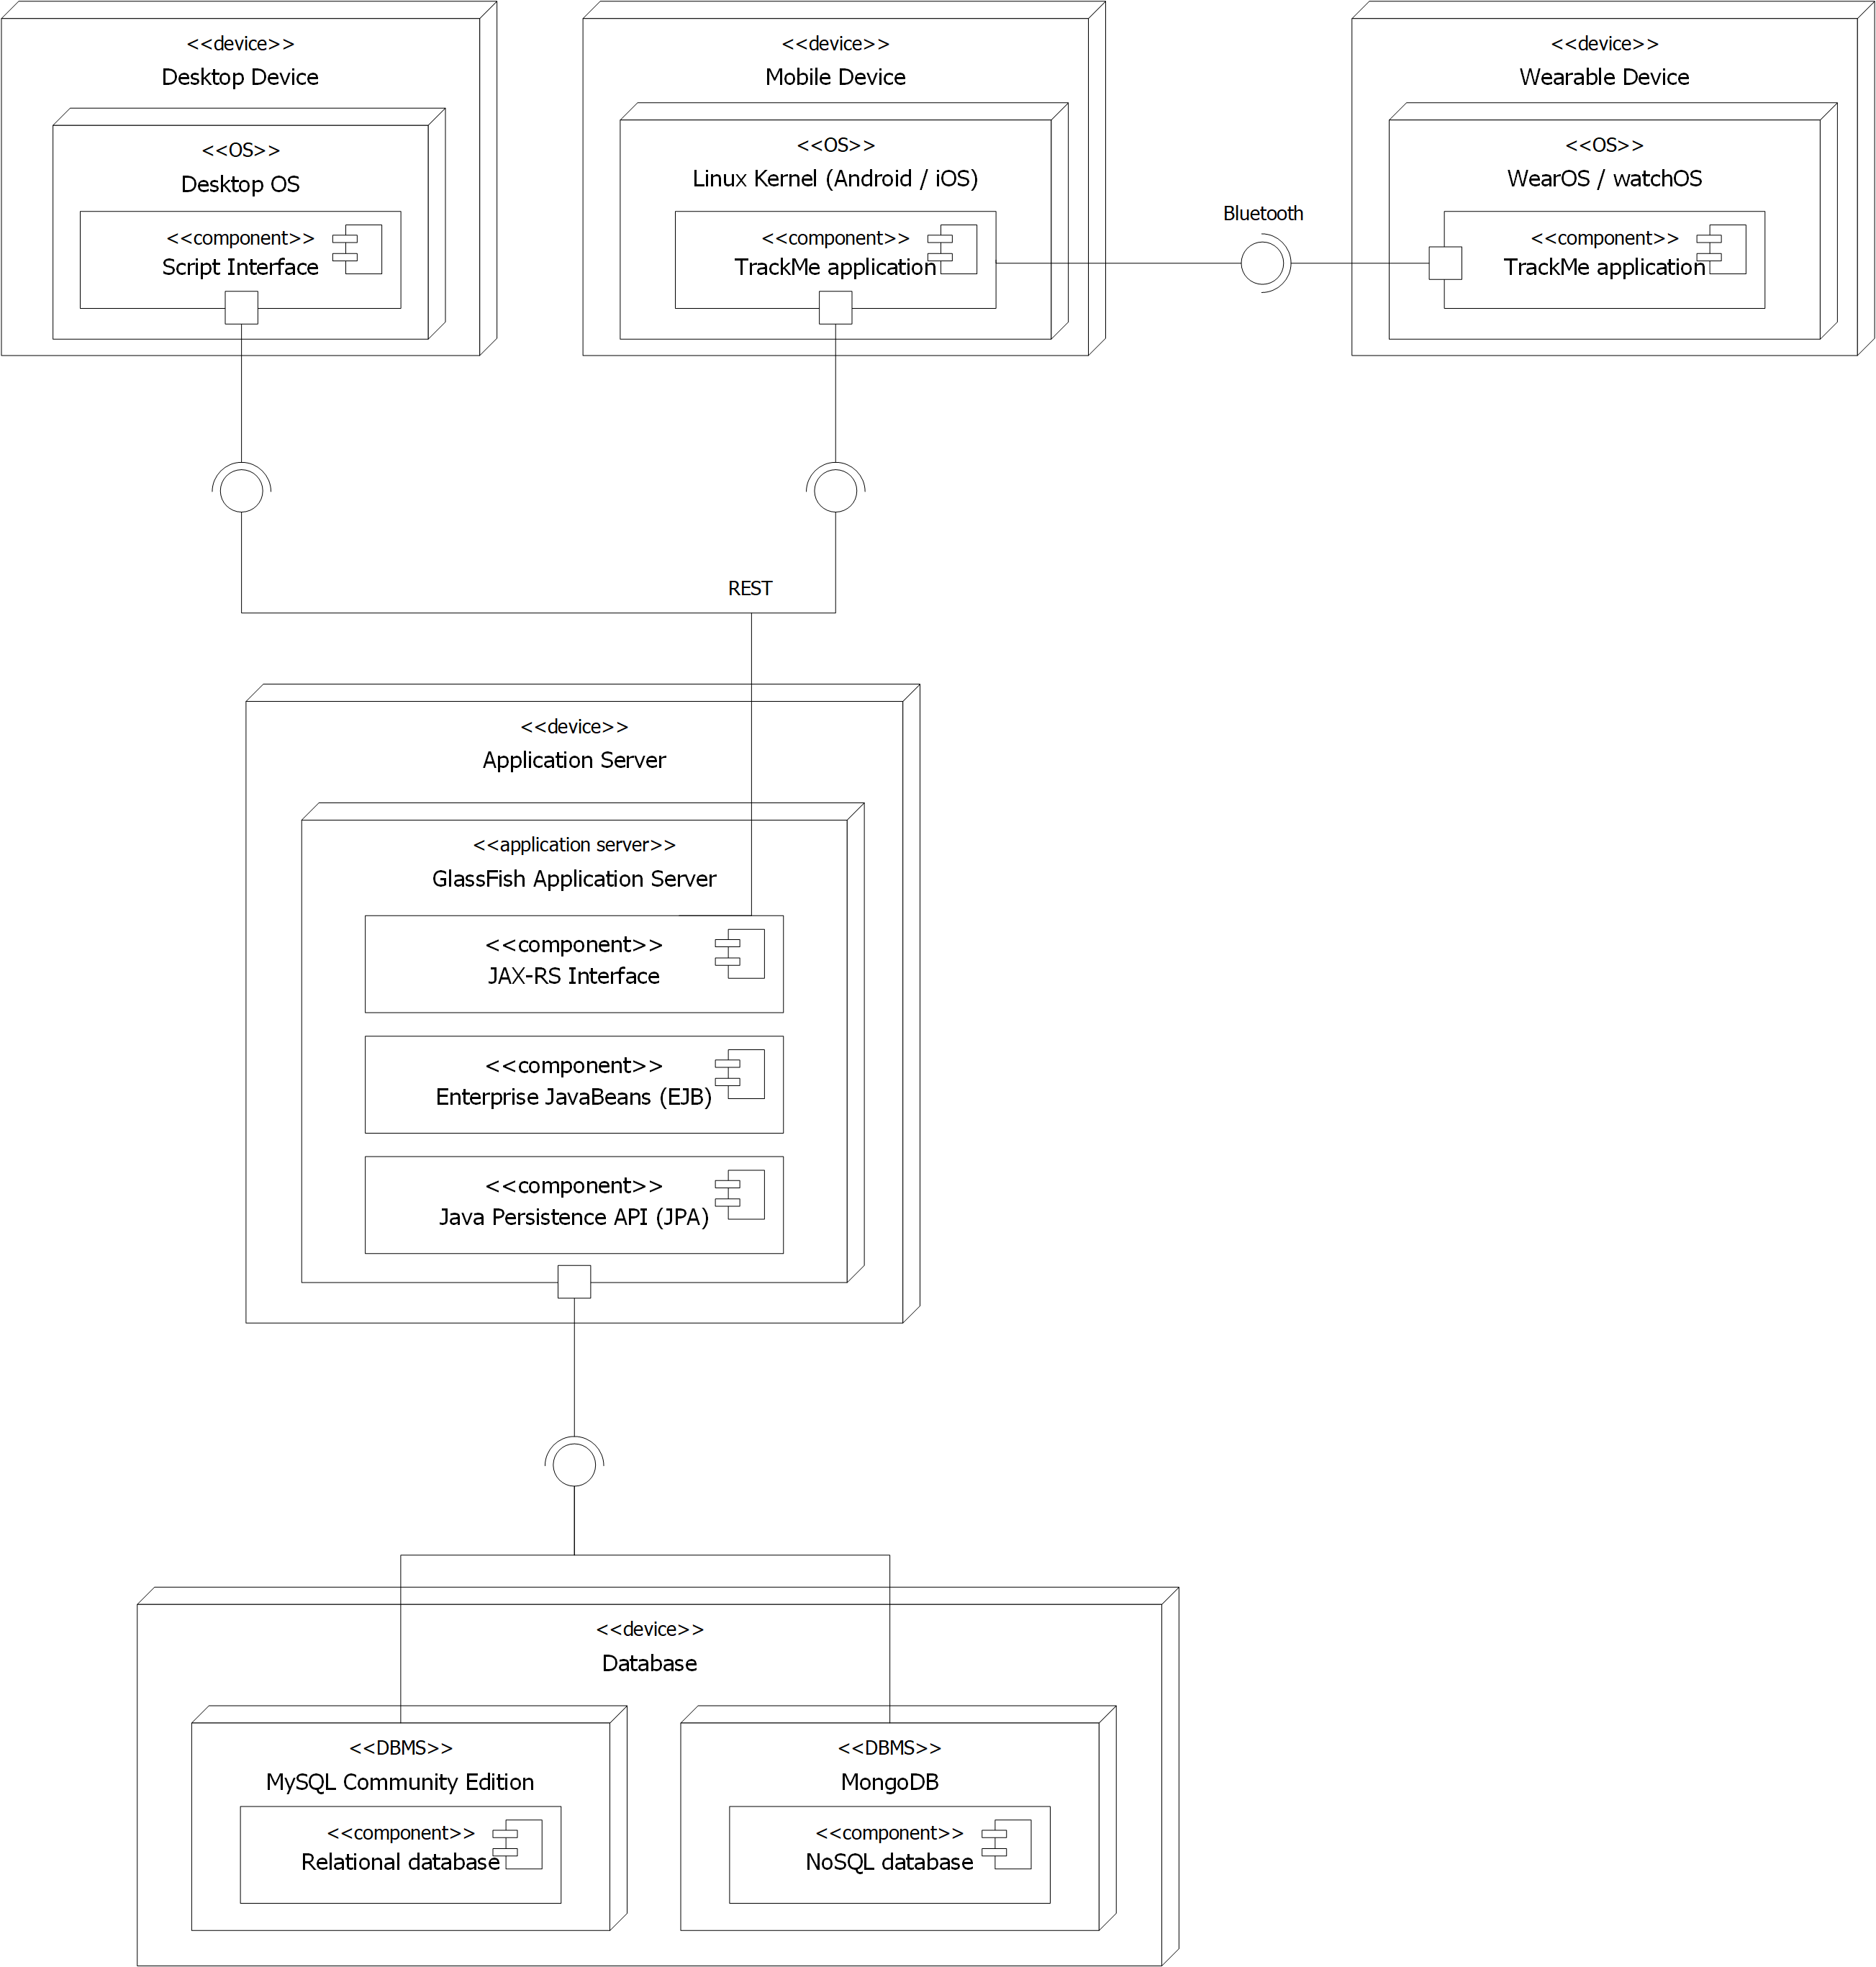
\includegraphics[scale=0.5]{sections/diagrams/deployment.png}
\newline
\captionof{figure}{Deployment diagram of the system}
\end{center}

\clearpage

\subsection{Runtime view}
In this section, a detail of the interactions between modules is shown. In particular, it is presented how the server modules, the clients and the database system interact at runtime in the most important scenarios as regarding main functionalities of the system.

The communication between the Application Server and the databases is abstracted by the Persistence Unit, so its data are represented with entity classes; the client is considered as a whole without dividing it into subcomponents.

\begin{center}
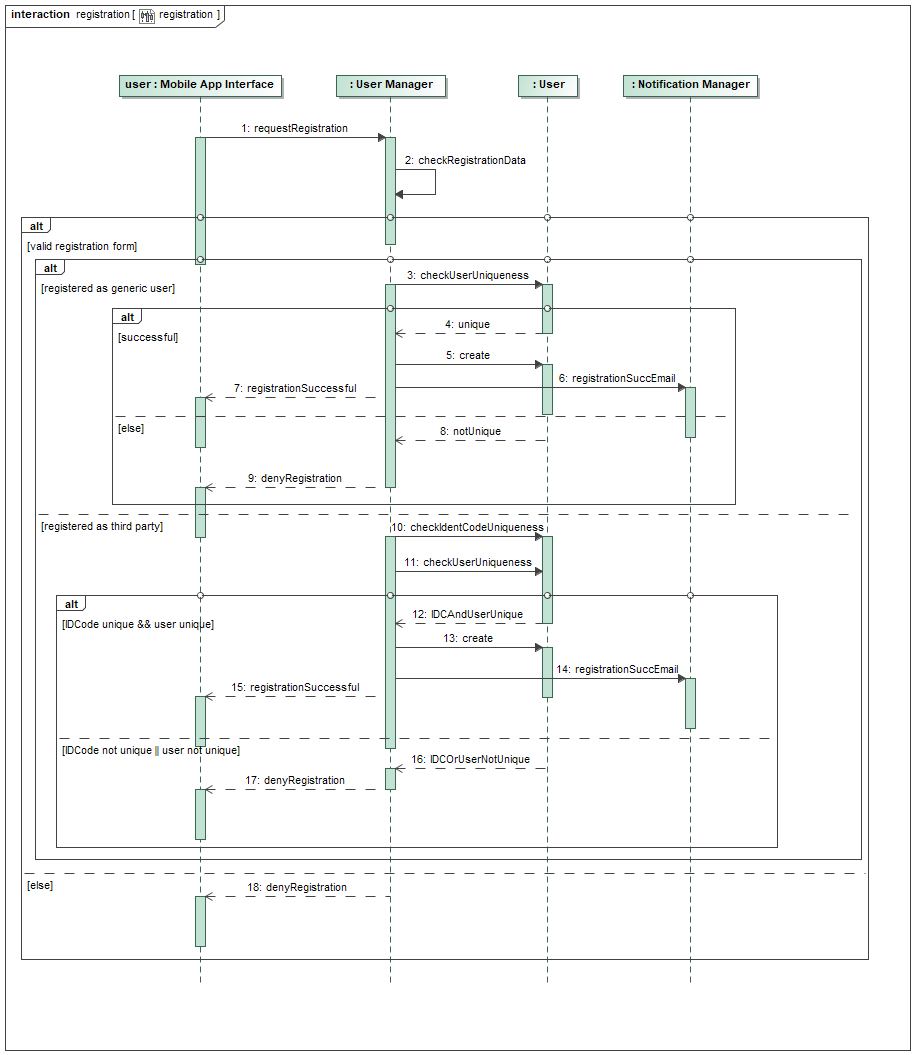
\includegraphics[scale=0.45]{sections/diagrams/registration}
\newline
\captionof{figure}{Sequence diagram of the steps to register to the application}
\end{center}

\begin{center}
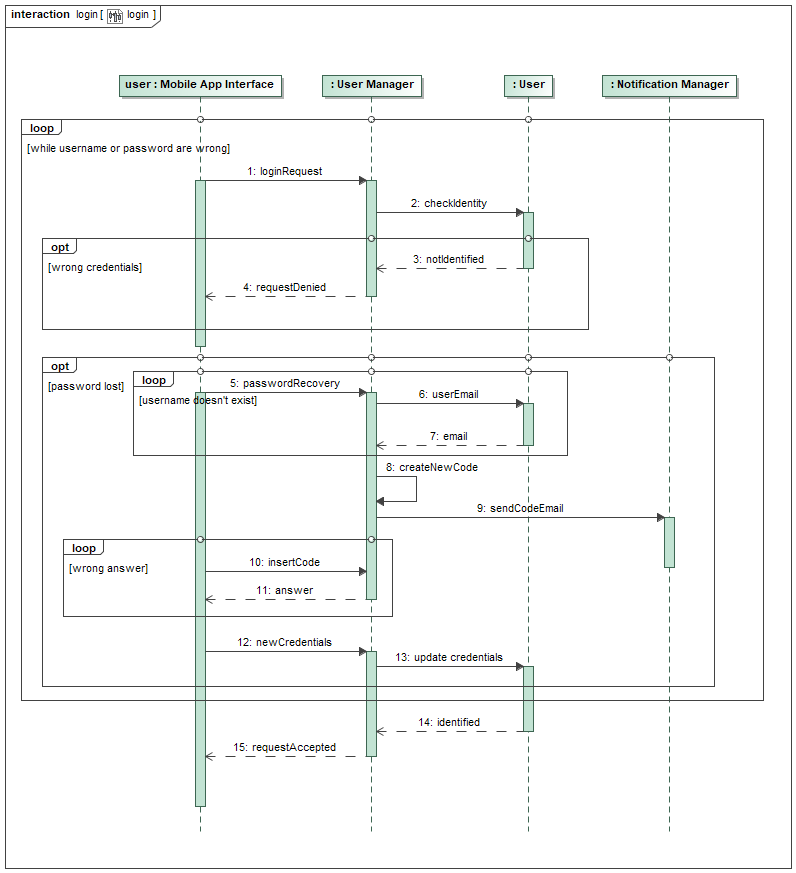
\includegraphics[scale=0.55]{sections/diagrams/login}
\newline
\captionof{figure}{Sequence diagram of the application login}
\end{center}

\begin{center}
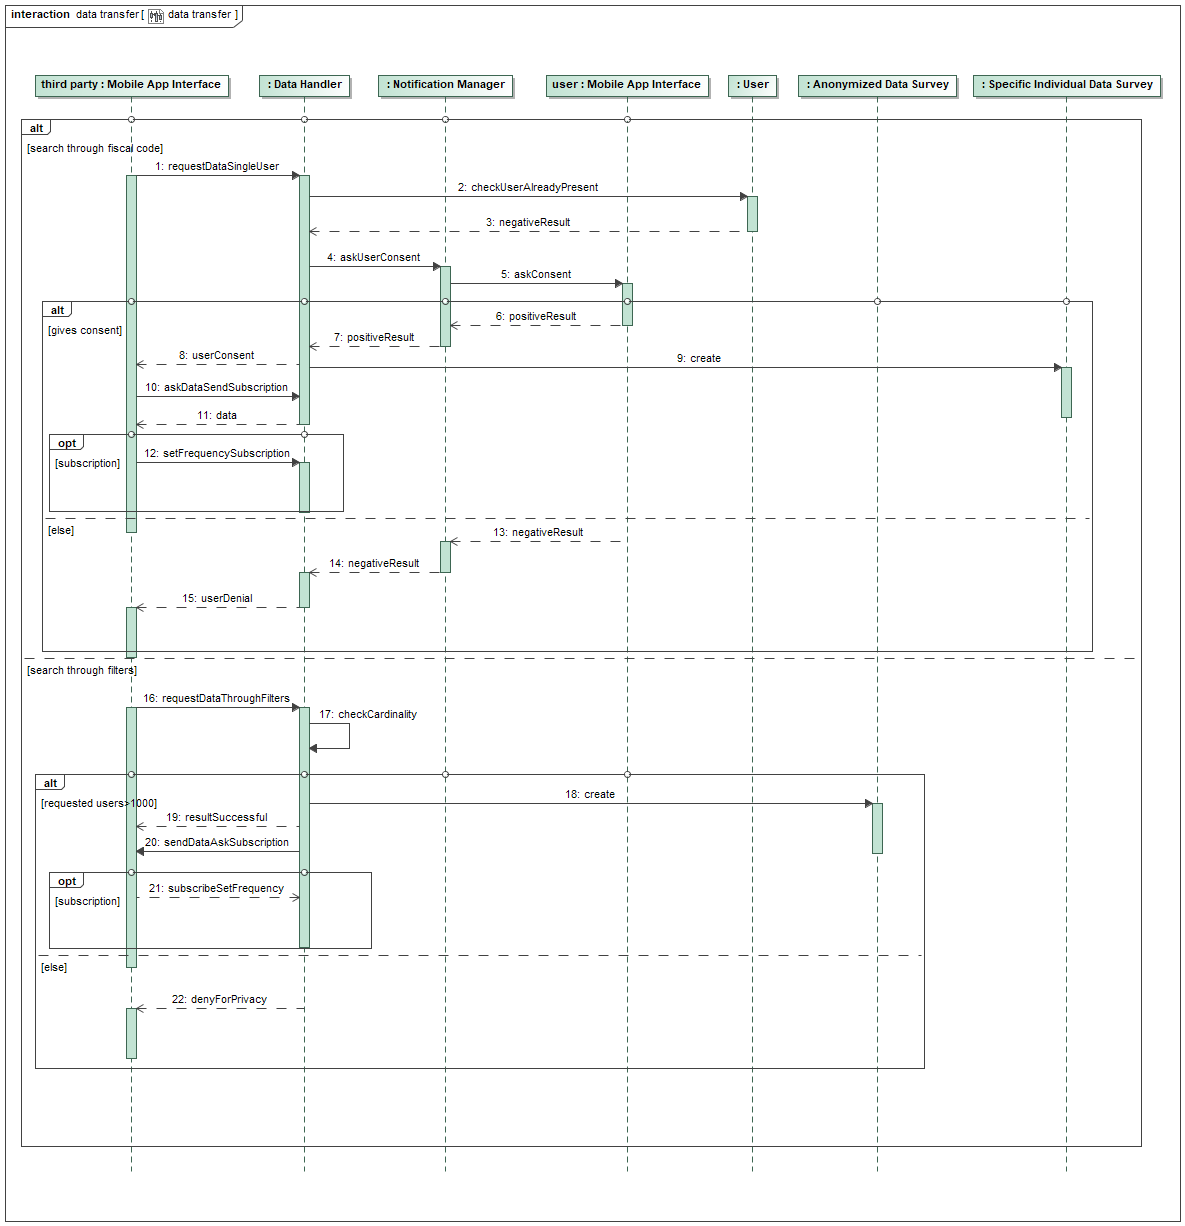
\includegraphics[scale=0.4]{sections/diagrams/data_transfer}
\newline
\captionof{figure}{Sequence diagram of a data request from a third party}
\end{center}

For sake of legibility in the previous sequence diagram only the case in which the third party doesn't have a survey with the searched user in it is shown. If the third party has already got it, the request for consent isn't forwarded, and the DataHandler gives directly the data requested with the possibility to subscribe to it. This fuctionality is given through the methods \texttt{askDataSendSubscription(subscription)} and \texttt{setFrequencySubscription(frequency)}, alrea\-dy shown in the diagram.

\begin{center}
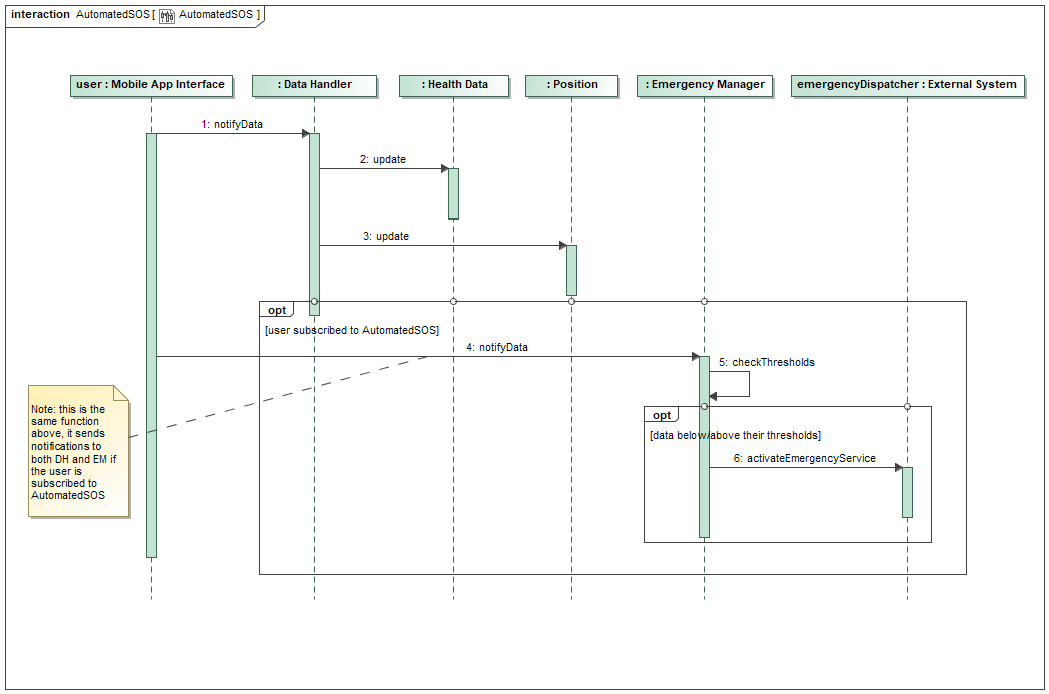
\includegraphics[scale=0.4]{sections/diagrams/AutomatedSOS}
\newline
\captionof{figure}{Sequence diagram of an emergency situation}
\end{center} 

\begin{center}
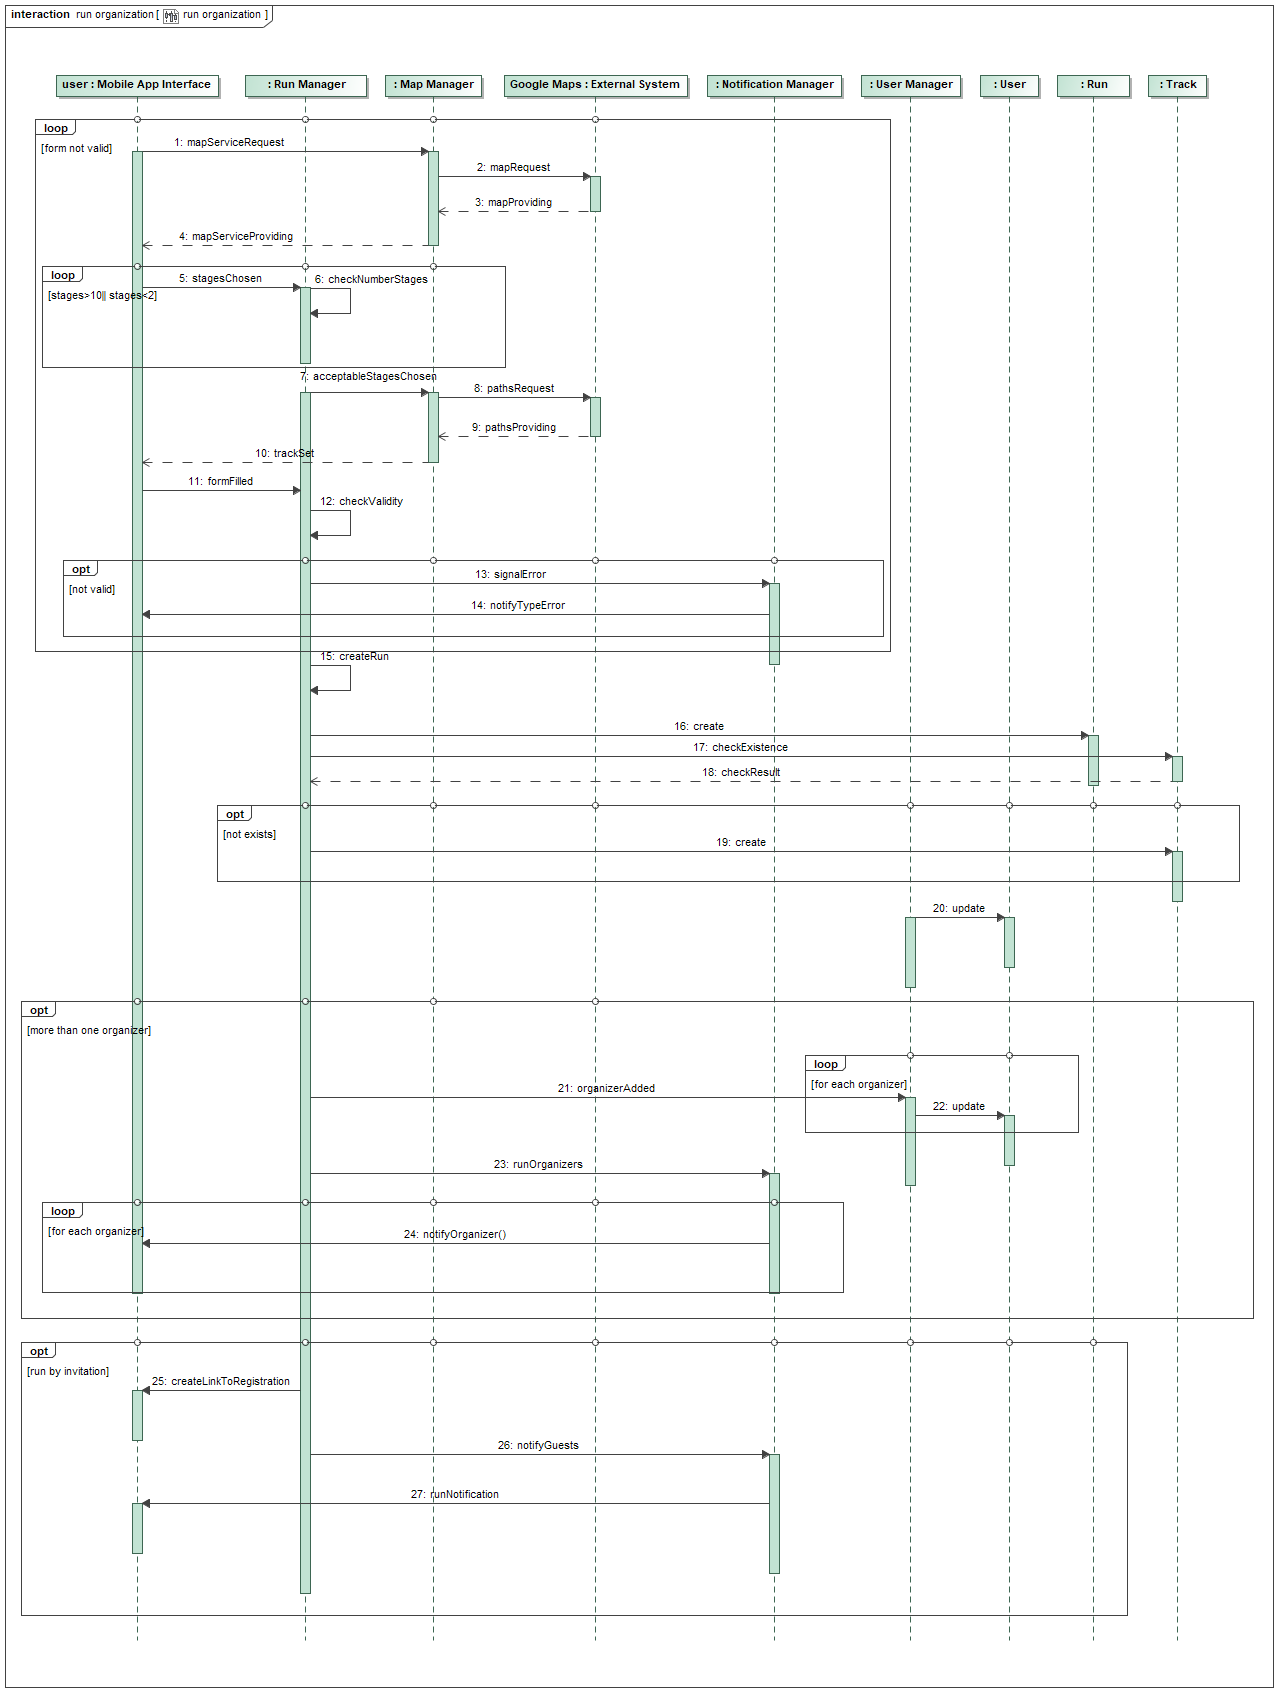
\includegraphics[scale=0.35]{sections/diagrams/run_organization}
\newline
\captionof{figure}{Sequence diagram of a run creation and organization}
\end{center}

\begin{center}
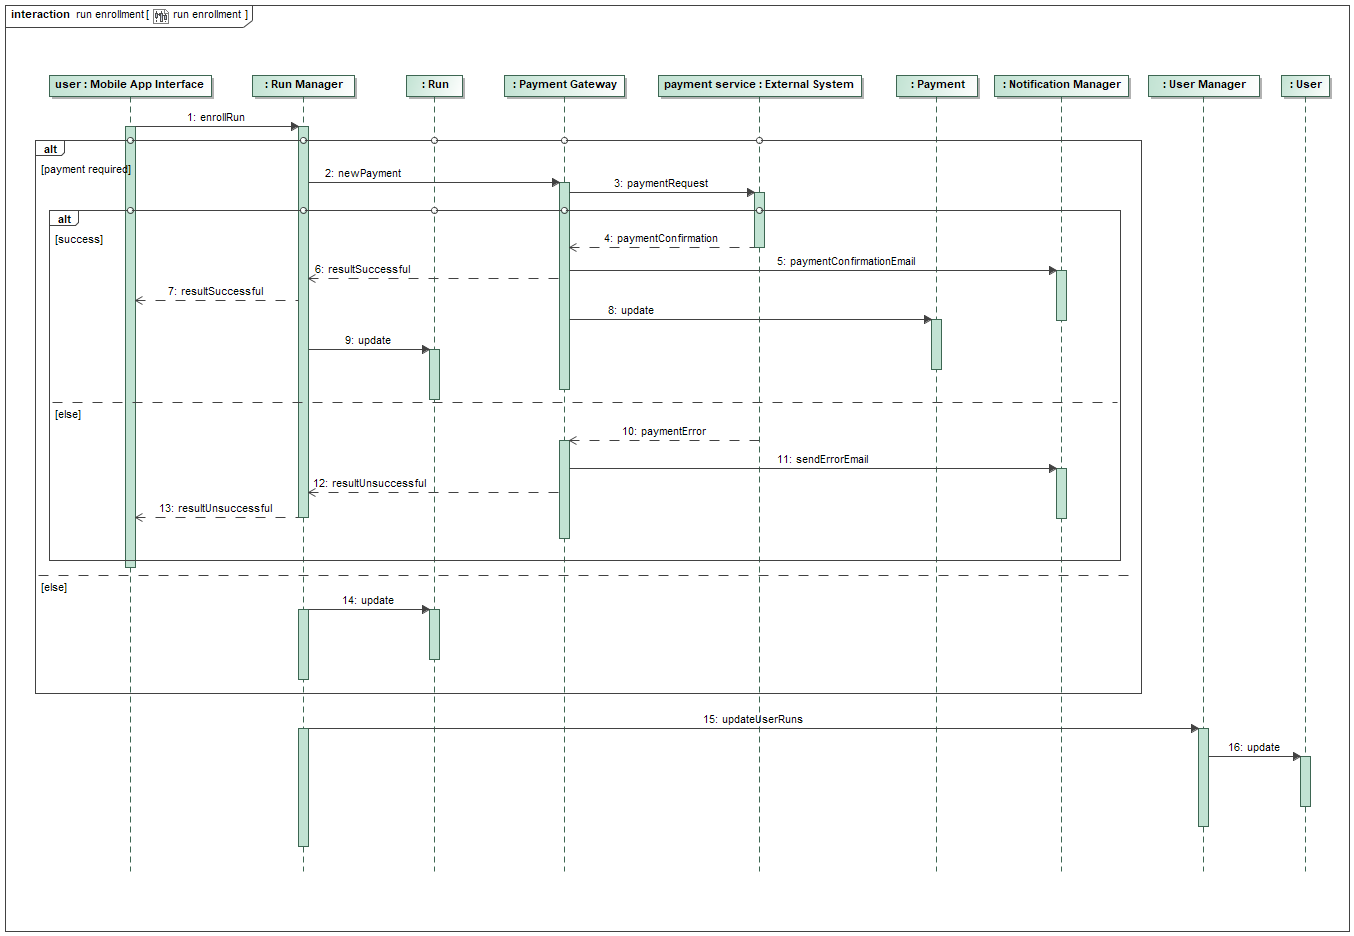
\includegraphics[scale=0.35]{sections/diagrams/run_enrollment}
\newline
\captionof{figure}{Sequence diagram of a run enrollment from a generic user}
\end{center}

\begin{center}
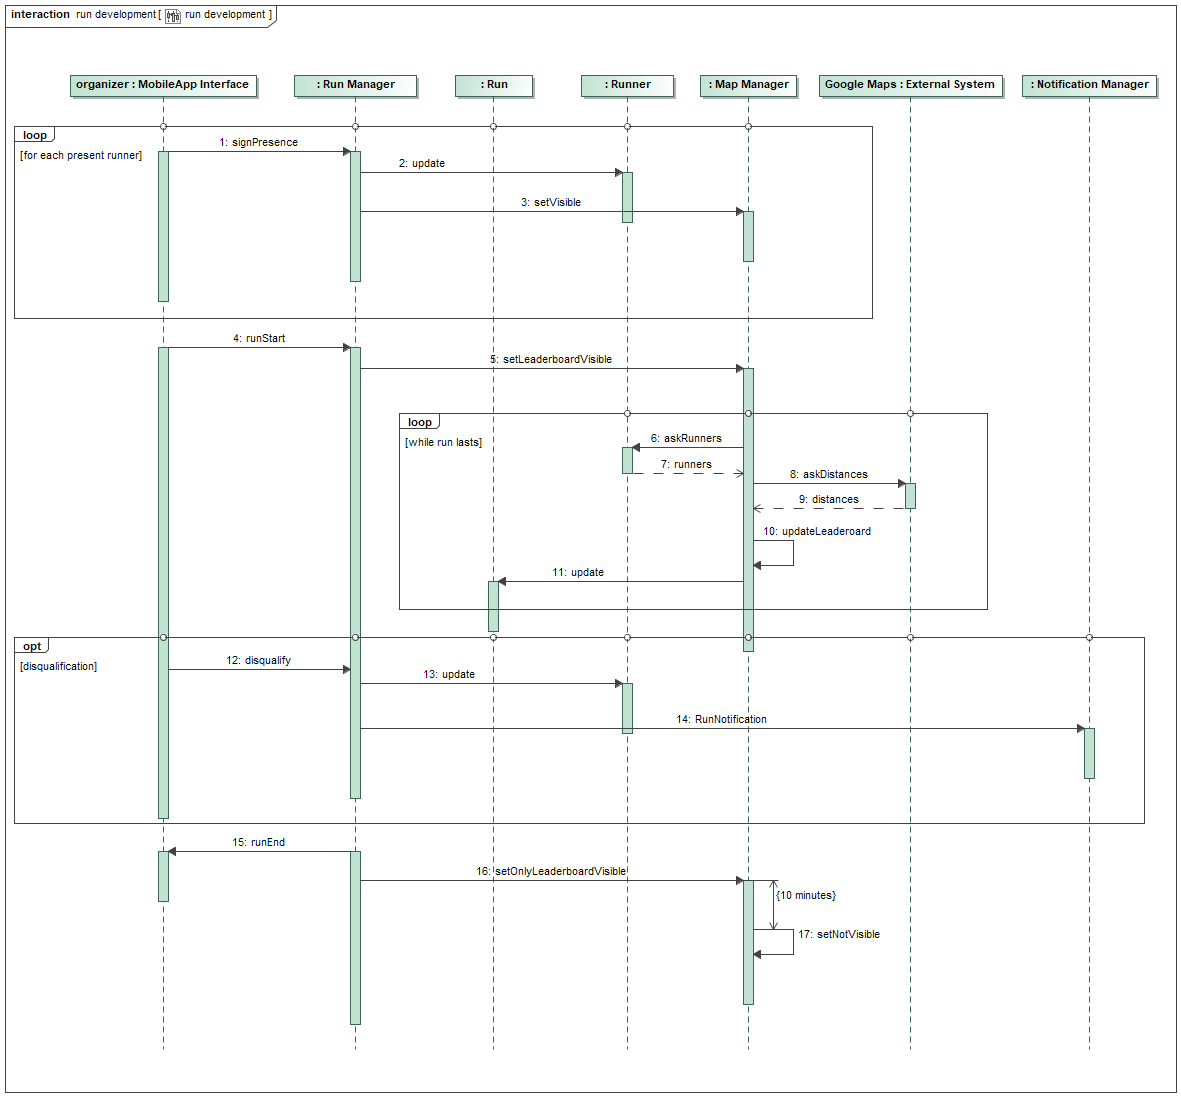
\includegraphics[scale=0.4]{sections/diagrams/run_development}
\newline
\captionof{figure}{Sequence diagram of a run development from its start to its end}
\end{center}

\subsection{Component interfaces}
This section deals with the comunication between components and subcomponents in terms of interfaces. In fact, the Application Server's interfaces will be described in detail in order to specify exactly how they can be used from the other components and server's subcomponents.

\subsubsection{Client}

The communication between Client (mobile application or script) and the Application Server is committed to RESTful APIs, that transmit data on HTTPS protocol without further levels. The communication itself is an exchange of HTTPS instructions, URLs and JSON objects.

\subsubsection{DBMSs}

Since data are mapped into JPA entities, they will be stored persistently in the two databases. The relational one uses JPA over SQL to communicate with the database, while the non relational one uses Eclipse JNoSQL APIs.
In order to reply to queries that require both the databeses content two or more distinct queries have to be merged on a more higher level. 


\subsubsection{External Systems}

As regards the mapping service, the Application Server must interface with Google Maps JavaScript API in order to display tracks and runners in real time and in a personalized way, SDK Maps for Android and SDK Maps for iOS, allow an easy way to configure and deploy location services on smartphone.

Payments are committed to a Payment Handler who will provide the appropriate APIs to manage payments of any kind. In particular, the system must support the main payment methods: PayPal and the main credit cards.

As already set in the RASD document, for notifications and messages the Application Server uses the Push Notifications Gateway of own APIs (Push API, to send notification when the application is closed) and a standard SMS \& Voice Gateway. 
An example could be Nexmo, with its SMS \& Voice API RESTful service.

Finally, applications that communicate with smart bands and wearable devices other than WearOS and watchOS are considered external systems. Therefore, they will provide their own APIs for communication with the Application Server.

\subsubsection{Interfaces of Application Server subcomponents}

\paragraph*{DataHandler}

\begin{itemize}
\item[ ]\texttt{requestDataSingleUser(fiscal code)}: method used to forward the request of data of a specific individual; it returns the reply (consent or deny).

\item[ ]\texttt{askDataSendSubscription(subscription)}: method used to ask the data requested and assert if he/she wants to subscribe to those data at the same time; it returns the health data and the position.

\item[ ]\texttt{setFrequencySubscription(frequency)}: method used to set the frequency on which the caller wants to receive the user's data; it returns nothing.

\item[ ]\texttt{requestDataThroughFilters(location, address, age, gender, timeSlot)}: method us\-ed to send, in order to submit to check, the request of data of an anonymized group of persons; it returns the check result (success/deny for privacy).

\item[ ]\texttt{checkCardinality(specifiedUsersList)}: method used to check if the considered group should be considered anonymized; it returns a boolean result.

\item[ ]\texttt{notifyData(user, healthData, position)}: method used to send data to the Data Handler module, that will store them in the NoSQL database: as already stated, only the Application Server can access the databases; it returns nothing.
\end{itemize}

\paragraph*{EmergencyManager}

\begin{itemize}
\item[ ]\texttt{notifyData(user, healthData, position)}: this method is the same above, it corresponds to the observer pattern's "update", but here it's used to send data in order to check if the user is in danger; it returns nothing.

\item[ ]\texttt{checkThresholds(healthData)}: method used to check if each type of health data stays between certain thresholds (which can be taken from health data themselves).
\end{itemize}

\paragraph*{MapManager}

\begin{itemize}
\item[ ]\texttt{mapServiceRequest(locationName)}: method used to forward a request for a map; it returns the requested map.

\item[ ]\texttt{acceptableStagesChosen(positionsSet)}: method used to forward a request for the shortest path between the stages selected; it returns the path.

\item[ ]\texttt{setRunnerVisible(), setLeaderBoardVisible(), setNotVisible(), setOnlyLeaderb\-oardVisible()}: these four methods are used to set what is visible on the screen of a run display; they return nothing.

\item[ ]\texttt{updateLeaderboard(distancesSet)}: method used to recalculate the leaderboard according to the new runners' distances from the end on the path; it returns the new leaderboard.
\end{itemize}
 
\paragraph*{NotificationManager}

\begin{itemize}
\item[ ]\texttt{askUserConsent(user, thirdParty)}: method used to send a notification through which is asked consent for a survey; it returns the user's reply (positive ore negative).

\item[ ]\texttt{signalError(user, type} method called when a component wants to send an error notification to the user, specifying the type of error; it returns nothing.

\item[ ]\texttt{runOrganizers(organizerList, run)}: method used when in the creation of a run more than one organizer are set and they need to be informed; it returns nothing.

\item[ ]\texttt{notifyGuests(runnersList, run)}: method used in order to command to send a notification to all the users invited to a private run; it returns nothing.

\item[ ]\texttt{runNotification(user, type)}: method used to create a notification for a runner, which message depends on the type of run notification; it returns nothing.

\item[ ]\texttt{paymentConfirmationEmail(user, paymentCode)}: method used to make the NotificationManager module send an e-mail of confirmation for the payment; it returns nothing.

\item[ ]\texttt{sendErrorEmail(user, paymentCode)}: method used to make NotificationManager send an e-mail to warn the user his/her payment wasn't successful; it returns nothing.

\item[ ]\texttt{registrationSuccEmail(user)}: method used to make NotificationManager send an e-mail to confirm the success of the registration operation; it returns nothing.

\item[ ]\texttt{sendCodeEmail(user, code)}: method used to make NotificationManager send an e-mail with an identification code in order to create a new password; it returns nothing.
\end{itemize}

\paragraph*{PaymentGateway}

\begin{itemize}
\item[ ]\texttt{newPayment(userCredentials, paymentMethod)}: method used to forward a payment request; it returns the payment result (successful or unsuccessful).
\end{itemize}

\paragraph*{RunManager}

\begin{itemize}
\item[ ]\texttt{stagesChosen(stagesSet)}: method used to send the track stages to submit to check; it returns nothing.

\item[ ]\texttt{checkNumberStages(stagesSet)}: method used to check if the number of stages exceeds 10; it returns the check result (positive or negative).

\item[ ]\texttt{formFilled(form)}: method used to send the run form filled out; it returns nothing.

\item[ ]\texttt{checkValidity(form)}: method used to check if the form is filled correctly and it's therefore possible to create the run; it returns the check result (positive or negative).
\end{itemize}

\paragraph*{UserManager}

\begin{itemize}
\item[ ]\texttt{requestRegistration(e-mail, username, password)}: method used to forward a request to register to the application, it returns the result (deny or success).

\item[ ]\texttt{checkregistrationData(form)}: method used to check if the registration form is complete and its fields have been completed in an acceptable way; it returns the check result.

\item[ ]\texttt{loginRequest(username, password)}: method used to require to be identified as a user already registered; it returns the result (deny or acceptance).

\item[ ]\texttt{passwordRetrieval(username)}: method used to ask for the possibility to use a new password; it returns nothing.

\item[ ]\texttt{createNewCode()}: method that create a temporary identification code in order to make the user choose his/her new password; it returns the code.

\item[ ]\texttt{insertCode(code)}: method called to send the code and to check if it matches the code generated previously by the UserManager module; it returns the check result (right or wrong).

\item[ ]\texttt{newCredentials(username, newPassword)}: method used to send the new password chosen by the user; it returns nothing.
\end{itemize}

\subsection{Selected architectural styles and patterns}
\subsubsection{Architectural Styles}
\paragraph*{Client and Server}
The main architectural style adopted for TrackMe system is the Client-Server one, the most well known and used architectural style for distributed applications. It will be adopted in the 3-tier variant, with the Presentation layer on the client (the mobile app), the Application layer on the Application Server and the Data layer on the Database Server.

The main advantages of this choice are the clear decoupling between data and logic, the possibility to increase the portability reaching clients in the most easy way and the availability of a lot of COTS components to  develop the system in a very cost-effective way.

\paragraph*{Layers}
The system will also be divided into 3 Layers:
\begin{itemize}
\item Presentation Layer: accessible from users through their mobile application.
\item Business Layer: it's on the Application Server.
\item Data Layer: it's on the Database Server.
\end{itemize}
Software is divided in layers for decoupling and for better code maintainability. In this way different developers can focus on different tasks abstracting from other layers.

\paragraph*{Thin Client}
The thin client approach has been followed while designing the interaction among users’ machines and the system itself. All the main logic is implemented by the Application Server that has a sufficient computing power and can manage concurrency issues in an efficient way. On the other hand, the mobile application are in charge of presentation only and they do not involve decision logic.

\subsubsection{Design Patterns}
\paragraph*{Model-View-Controller}
The mobile (and wearable) application follow the MVC (Model-View-Controller) software design pattern, that better supports the Client-Server architecture, because it closely follows the division between data (Model), logic (Controller) and presentation (View) present also in our 3-tier architecture.

\paragraph*{Observer}
The observer or publish-subscribe pattern will also be used, allowing the various components of the system to register themselves and react to event raised by other components. This will be useful in implementing the EmergencyManager that always has to be notified in order to compare data and thresholds.

\subsection{Other design decisions}
\subsubsection{Passwords storage}
For security reasons, the user’s password is stored using cryptographic hash functions. In addition to that, the password is not only hashed, but also salted. This is a common security choice since many users reuse passwords for multiple sites and a cyber-attack could jeopardize their sensitive information.

%\end{document}